\chapter{Equations générales de cinématique des fluides}
Ce petit chapitre présente quelques équations générales valables quelle que
soit la loi de comportement (fluides parfaits/visqueux).

\section{Le tourbillon}
Le champ de tourbillon est défini par $\vec{\omega} = \frac{1}{2}\rot \vec{v}$ 
ou encore en notation indicielle : $\omega_i = \frac{1}{2}\delta_{ijk}\partial_j
v_k$. Si $\omega$ est un rotationnel, sa divergence est forcément nulle :
\begin{equation}
	\text{div}\ \vec\omega = 0\ \ \ \ \text{ou }\ \ \ \omega_{i,i} = 0
\end{equation}
En passant l'intégrale de part et d'autre et après application du théorème de 
Gauss, le tourbillon est dit "conservatif" : 
\begin{equation}
	\int_v \omega_{i,i}\ dV = 0 \Rightarrow \oint_S \omega_i\ n_i\ dS = 0
\end{equation}
c'est-à-dire que le flux de tourbillon au travers d'une surface fermé est 
nul\footnote{Ce qui rentre est égal à ce qui sort.}.

\subsection{Tube de tourbillon}
Un peu de vocabulaire pour le bien de tous :
\begin{description}
	\item[Ligne de tourbillon] : courbe enveloppe du vecteur tourbillon.
	\item[Surface de tourbillon] : surface engendrée par les lignes de 
	tourbillon s'appuyant sur une courbe quelconque.
	\item[Tube de tourbillon] : surface engendrée par une courbe fermée (
	\textit{filament de tourbillon} si la courbe est "élémentaire")
\end{description}
Le tube de tourbillon fonctionne exactement comme celui de courant si ce 
n'est qu'ici c'est le vecteur tourbillon qui est parallèle à la surface 
latérale.
	
\subsubsection{Filament de tourbillon}
On imagine un tuyau d'arrosage qui au lieu de conduire l'eau, conduit 
des tourbillons. Ainsi, exactement comme pour le tube de courant :
\begin{equation}
	\omega'S' = \omega''S''
\end{equation}
car la vecteur tourbillon est tangent à la surface latérale $\Sigma$.\\
\begin{center}
	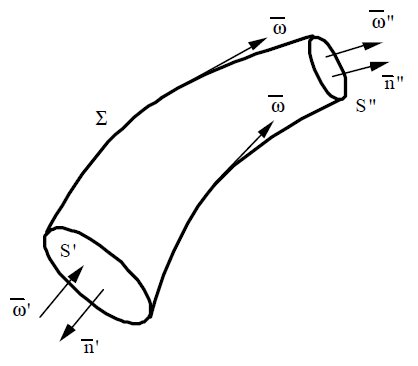
\includegraphics[scale = 0.4]{ch8/1}
	\captionof{figure}{Tube de tourbillon}
\end{center}
		
\subsubsection{Tube de tourbillon}
Comme précédement mais pour le tourbillon :
\begin{equation}
	\int_S \omega.\vec{n}\ dS = C^{ste}
\end{equation}
pour toute section $S$ du tube de tourbillon.
		
		
\subsubsection{Circulation de la vitesse}
Considérons une section dans un tube de tourbillon : on obtient une
surface $S$ limitée par la courbe fermée $\mathcal{C}$. Le long de cette 
section constante, on considère le vecteur $\vec{dL}$ tangent à cette courbe 
pour en calculer l'intégrale suivante, donnant la circulation de la vitesse 
le long de la courbe fermée $\mathcal{C}$ :
\begin{equation}
	\Gamma = \oint_\mathcal{C} \vec{v}.\vec{dL}
\end{equation}
Appliquons le théorème de Stokes :
\begin{equation}
	\Gamma = \oint_\mathcal{C} \vec{v}.\vec{dL} = \int_S \rot \vec{v}.\vec{n}\ dS
\end{equation}
On obtient alors :
\begin{equation}
	\Gamma = \int_S 2\vec{\omega}.\vec{n}\ dS = C^{ste}
\end{equation}
Ceci montre que cette intégrale est constante : la circulation $\Gamma$ de la 
vitesse le long d'une courbe fermée $\mathcal{C}$ sur un tube de tourbillon est 
une constante quelle que soit la section.\\
\begin{center}
	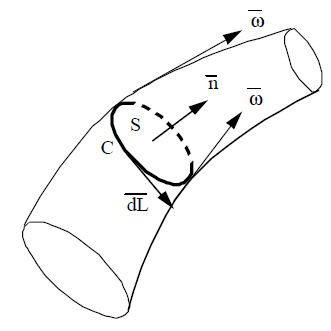
\includegraphics[scale = 0.4]{ch8/2}
	\captionof{figure}{Circulation de la vitesse}
\end{center}